%%%%%%%%%%%%%%%%%%%%%%%%%%%%%%%%%%%%%%%%%
% GNet - Poster zum BWKI-Finale (A0 hochkant)
% Vorlage: a0poster Portrait Poster for LiRI/UZH (CC BY-NC-SA 3.0),
%   Kettl & Weiser, angepasst von Danny McDonald
% Kompilieren: xelatex main.tex  (fontspec)
% Bilder/Daten: python make_figures.py  ->  figures/
%%%%%%%%%%%%%%%%%%%%%%%%%%%%%%%%%%%%%%%%%

\documentclass[a0,portrait]{a0poster}

\usepackage{geometry}
 \geometry{
 a0paper,
 hoffset=0pt, voffset=0pt, % a0poster verschiebt sonst alles um ca. 1 Zoll nach links oben
 left=3cm,
 top=2.5cm,
 right=3cm,
 bottom=1.6cm
 }

\usepackage[svgnames]{xcolor}
\definecolor{uzhockerrot100}{RGB}{220, 96, 39}
\definecolor{uzhflaschengruen100}{RGB}{42, 127, 98}
\definecolor{bwkiblau}{HTML}{0083D3}
\definecolor{conclusion}{HTML}{D6ECF8}
\definecolor{rulegray}{RGB}{203,213,225}
\definecolor{textgray}{RGB}{71,85,105}
\definecolor{blausoft}{HTML}{E8F4FB}
% Aufgaben in Tab. 1
\definecolor{tFhBg}{HTML}{E8F4FB}  \definecolor{tFhFg}{HTML}{0083D3}   % GLips-500
\definecolor{tFzBg}{HTML}{E6F4EF}  \definecolor{tFzFg}{RGB}{42,127,98}  % GLips-15
\definecolor{tTrBg}{HTML}{FCEDE5}  \definecolor{tTrFg}{RGB}{220,96,39}  % GLips-15 + Transfer
% Fusionssysteme
\definecolor{cA}{RGB}{0, 40, 165}     % Joint Transformer
\colorlet{cB}{uzhockerrot100}         % Cross-Attention
\colorlet{cC}{uzhflaschengruen100}    % Concat
\definecolor{cD}{RGB}{224,161,0}      % nur Audio
% Modelle in den Kurven
\colorlet{cGNet}{bwkiblau}
\colorlet{cMSTCN}{uzhockerrot100}
% Bausteine im Architekturdiagramm
\definecolor{mConv}{HTML}{2B7BD1}
\definecolor{mPool}{HTML}{E0403A}
\definecolor{mTemp}{HTML}{5B4FD6}
\definecolor{mAttn}{HTML}{F08A00}
\definecolor{mAudio}{HTML}{C2378F}
\definecolor{mFC}{HTML}{2EA043}

\usepackage{graphicx}
\graphicspath{{figures/}{./}}
\usepackage{booktabs}
\usepackage{colortbl}
\usepackage[font=footnotesize,labelfont=bf]{caption}
\captionsetup{skip=0.5cm}
\usepackage{amsmath}
\usepackage{tikz}
\usetikzlibrary{positioning, arrows.meta, fit, calc, backgrounds}
\usepackage{pgfplots}
\usepgfplotslibrary{groupplots}
\pgfplotsset{compat=1.18}
\usepackage[ngerman]{babel}

\usepackage{fontspec}
\defaultfontfeatures[TheSans]
{
    Extension = .otf,
    UprightFont = font/TheSans-LP5Plain,
    BoldFont = font/TheSans-LP7Bld,
    ItalicFont  = font/TheSans-LP5PlainIT,
    BoldItalicFont = font/TheSans-LP7BldIT,
}
\IfFileExists{font/TheSans-LP5Plain.otf}{\setmainfont{TheSans}}{\setmainfont{Arial}} % UZH-Schrift, sonst Arial
\usepackage{unicode-math}
\setmathfont{latinmodern-math.otf}
\setmathfont{Arial}[range={up/num, up/latin, up/Latin}]
\setmathfont{Arial Italic}[range={it/latin, it/Latin}]
\usepackage{setspace}
\setstretch{1.1}
\usepackage{tcolorbox}
\usepackage{enumitem}
\setlist{itemsep=0.4ex, topsep=0.4ex, parsep=0pt, leftmargin=1.1em}

\newcommand{\best}[1]{{\color{bwkiblau}\textbf{#1}}}
\arrayrulecolor{rulegray}
\pgfplotsset{
  every axis/.append style={
    font=\footnotesize, tick label style={font=\footnotesize, color=textgray},
    label style={font=\footnotesize},
    /pgf/number format/use comma, /pgf/number format/assume math mode=true,
    axis line style={draw=rulegray}, tick style={draw=none},
    ymajorgrids, major grid style={draw=rulegray!70},
    title style={font=\small\bfseries},
  },
  % horizontale Balken, eine Serie pro Farbe, keine Gruppierung
  hbars/.style={
    xbar, bar shift=0pt, bar width=8mm, scale only axis,
    ymajorgrids=false, xmajorgrids, y axis line style={draw=none},
    y tick label style={font=\footnotesize, color=black, align=right},
  },
  vals/.style={
    nodes near coords, nodes near coords style={font=\footnotesize\bfseries, anchor=west, color=black},
    every node near coord/.append style={/pgf/number format/.cd, fixed, fixed zerofill, precision=1, use comma},
  },
}
\setlength{\parindent}{0pt}
\setlength{\parskip}{0.4ex}

% ---------- Abschnitte: volle Breite, Linie + Nummer ----------
\newcounter{psec}
\newcommand{\psection}[1]{%
  \par\vspace{0.6cm}\stepcounter{psec}%
  \noindent{\color{bwkiblau}\rule{\linewidth}{3pt}}\par\vspace{0.35cm}%
  \noindent{\color{bwkiblau}\fontsize{46pt}{50pt}\selectfont\bfseries\thepsec.\hspace{0.5em}#1}\par\vspace{0.45cm}}
\newcommand{\phead}[1]{{\color{bwkiblau}\normalsize\bfseries #1}\par\vspace{0.2cm}}

% ---------- 3D-Quader fürs Architekturdiagramm ----------
% \cube{Name}{x}{y-Mitte}{Breite}{Höhe}{Tiefe}{Farbe}
\newcommand{\cube}[7]{%
  \pgfmathsetmacro\cdx{0.55*#6}\pgfmathsetmacro\cdy{0.42*#6}%
  \pgfmathsetmacro\cyb{#3-#5/2}\pgfmathsetmacro\cyt{#3+#5/2}\pgfmathsetmacro\cxr{#2+#4}%
  \filldraw[draw=#7!80!black, fill=#7!14!white, line width=1.1pt, line join=round]
    (#2,\cyt) -- ++(\cdx,\cdy) -- ++(#4,0) -- (\cxr,\cyt) -- cycle;
  \filldraw[draw=#7!80!black, fill=#7!42!white, line width=1.1pt, line join=round]
    (\cxr,\cyb) -- ++(\cdx,\cdy) -- ++(0,#5) -- (\cxr,\cyt) -- cycle;
  \filldraw[draw=#7!80!black, fill=#7!26!white, line width=1.1pt, line join=round]
    (#2,\cyb) rectangle (\cxr,\cyt);
  \coordinate (#1-w) at (#2,#3);
  \coordinate (#1-e) at ({\cxr+\cdx/2},{#3+\cdy/2});
  \coordinate (#1-n) at ({#2+#4/2+\cdx/2},{\cyt+\cdy});
  \coordinate (#1-s) at ({#2+#4/2},\cyb);
}

\begin{document}
\small

%----------------------------------------------------------------------------------------
%	KOPF
%----------------------------------------------------------------------------------------
\begin{center}
  {\color{bwkiblau}\fontsize{150pt}{150pt}\selectfont\bfseries German Lipnet}\\[0.6cm]
  {\fontsize{40pt}{48pt}\selectfont Audio-visuelles Lippenlesen auf Deutsch: bestes berichtetes Ergebnis auf GLips-15}\\[0.8cm]
  {\large\textbf{Peter Staykov, Dorian Benbassat, Konstantin Borodulin}}\\[0.2cm]
  {\normalsize Bundeswettbewerb Künstliche Intelligenz 2026}
\end{center}

%----------------------------------------------------------------------------------------
\psection{Datensatz und Vorverarbeitung}
%----------------------------------------------------------------------------------------
\noindent\begin{minipage}[t]{0.29\linewidth}\vspace{0pt}
\textbf{GLips} (Schwiebert et al., LREC 2022) besteht aus Reden im \textbf{Hessischen Landtag}.
Jeder Clip zeigt ein Wort aus einer echten Plenarrede: 1,16\,s, 29 Frames bei 25\,fps, mit
Tonspur. Den veröffentlichten Split mit 400/50/50 Clips pro Wort verwenden wir unverändert.


Insgesamt rund 250.000 Clips zu 500 Wörtern aus 1.018 Sitzungsvideos. Für den Vergleich mit
Vorarbeiten nutzen wir zusätzlich die 15-Wort-Teilmenge von Ameer et al.\ (2025).

\vspace{0.6cm}
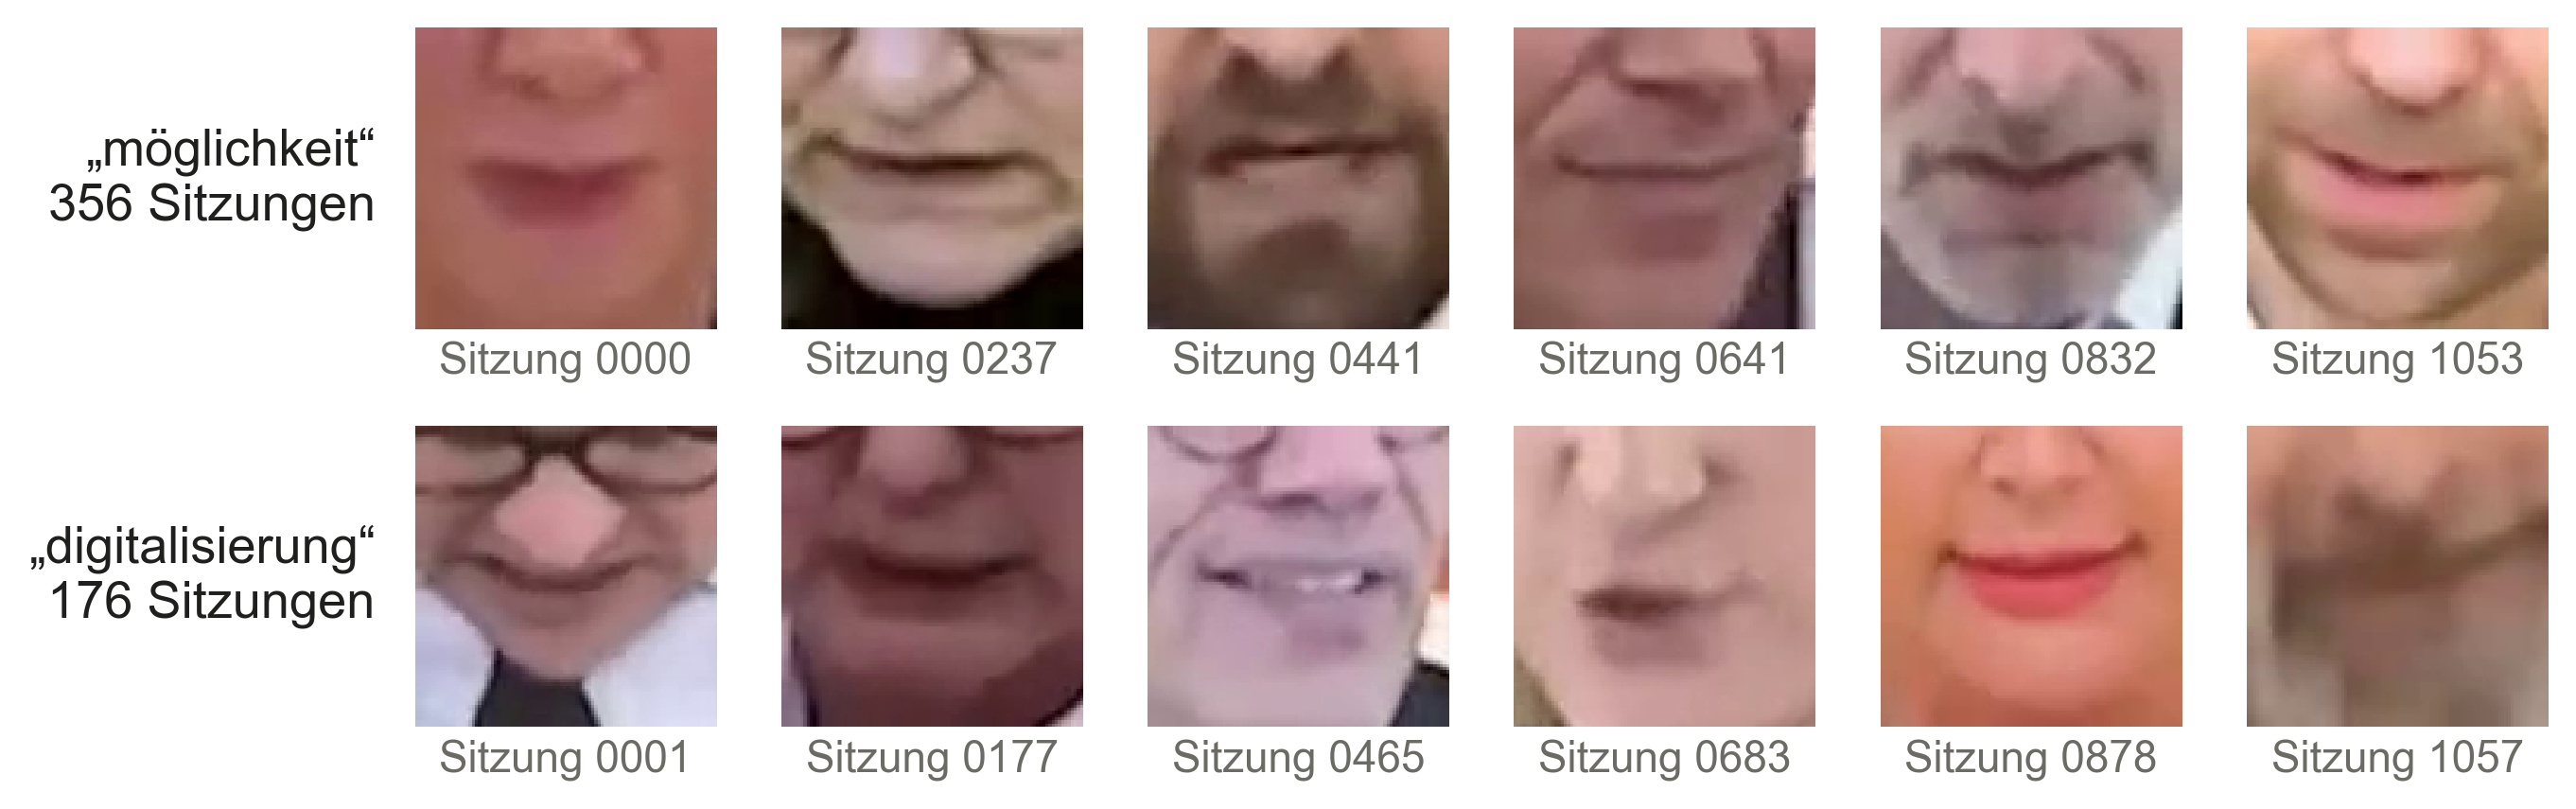
\includegraphics[width=\linewidth]{source_samples.png}
\captionof{figure}{Dasselbe Wort aus verschiedenen Sitzungen: Sprecher, Licht und
Bildqualität variieren stark.}

\vspace{0.7cm}
{\footnotesize\color{textgray}\textbf{GLips-15:} aber, aufgaben, bleibt, darüber, digitalisierung,
einmal, finden, gegen, geworden, herrn, investitionen, kommunen, linke, möglichkeit, passiert}
\end{minipage}\hfill
\begin{minipage}[t]{0.685\linewidth}\vspace{0pt}
\phead{Beispielclips nach dem Mund-Zuschnitt (je 6 von 29 Frames)}
\begin{tikzpicture}[x=1cm, y=1cm]
  \def\fw{4.0}\def\fg{0.18}
  \foreach \w/\word in {0/digitalisierung, 1/möglichkeit} {
    \pgfmathsetmacro\xx{\w*(6*(\fw+\fg)+1.3)}
    \node[anchor=south west, font=\small\itshape, text=black!80, inner sep=0] at (\xx,0.25) {„\word“};
    \foreach \k in {0,...,5} {
      \pgfmathtruncatemacro\f{2*\k}
      \node[inner sep=0, anchor=north west] at ({\xx+\k*(\fw+\fg)},0) {\includegraphics[width=\fw cm]{strip\w_\f.png}};
    }
    \draw[-{Stealth[length=5mm]}, line width=2pt, textgray] (\xx,-\fw-0.45) -- ({\xx+6*(\fw+\fg)-\fg},-\fw-0.45)
      node[pos=0.5, below=1mm, font=\footnotesize, text=textgray] {Zeit, 1,16\,s};
  }
\end{tikzpicture}

\vspace{0.5cm}
\phead{Vorverarbeitung}
\resizebox{\linewidth}{!}{%
\begin{tikzpicture}[x=1cm, y=1cm,
    arr/.style={-{Stealth[length=7mm, width=6mm]}, line width=2.6pt, draw=black!60},
    ttl/.style={font=\large\bfseries, anchor=south, align=center},
    dsc/.style={font=\normalsize, text=textgray, anchor=north, align=center, text width=15cm},
    img/.style={inner sep=0, draw=black!60, line width=1.2pt},
  ]
  % 1 Rohclip
  \node[img] (raw) at (5,0) {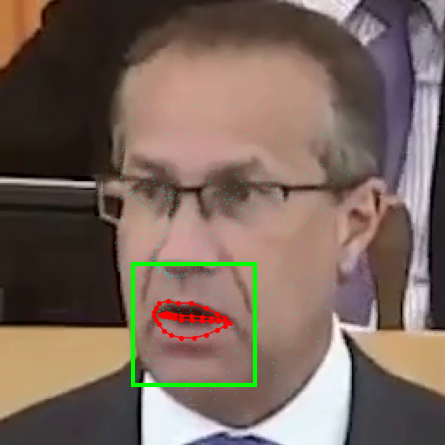
\includegraphics[width=10cm]{face_landmarks.png}};
  \node[ttl] at ([yshift=4mm]raw.north) {1\enspace Rohclip};
  \node[dsc] at ([yshift=-5mm]raw.south) {ganzes Gesicht,\\ 29 Frames, 25\,fps};
  % 2 FaceMesh
  \begin{scope}[shift={(19,0)}]
    \node[draw=black!60, line width=1.2pt, minimum size=10cm, fill=blausoft] (mesh) at (0,0) {};
    \foreach \a in {0,15,...,345} {
      \fill[mPool] ({3.3*cos(\a)},{1.25*sin(\a)+(\a>180?0.55:0)*sin(\a)}) circle (1.6mm);
      \fill[mPool] ({2.0*cos(\a)},{0.35*sin(\a)}) circle (1.3mm);
    }
    \draw[mPool, line width=1.4pt] plot[smooth cycle, domain=0:345, samples=24] ({3.3*cos(\x)},{1.25*sin(\x)+(\x>180?0.55:0)*sin(\x)});
    \draw[mPool, line width=1.2pt] plot[smooth cycle, domain=0:345, samples=24] ({2.0*cos(\x)},{0.35*sin(\x)});
    \draw[uzhflaschengruen100, line width=3pt] (-4.4,-4.4) rectangle (4.4,4.4);
    \draw[<->, line width=1.5pt, textgray] (-3.3,-2.6) -- node[below, font=\normalsize] {Mundbreite $b$} (3.3,-2.6);
    \draw[<->, line width=1.5pt, uzhflaschengruen100] (-4.4,3.4) -- node[below, font=\normalsize] {$1{,}6\,b$} (4.4,3.4);
  \end{scope}
  \node[ttl] at ([yshift=4mm]mesh.north) {2\enspace MediaPipe FaceMesh};
  \node[dsc] at ([yshift=-5mm]mesh.south) {Lippenlandmarken pro Frame,\\ Quadrat mit $1{,}6 \times$ Mundbreite};
  % 3 Glättung
  \begin{scope}[shift={(33,0)}]
    \node[draw=black!60, line width=1.2pt, minimum size=10cm] (ema) at (0,0) {};
    \draw[textgray, line width=1.2pt, -{Stealth}] (-4.3,-4.2) -- (4.4,-4.2) node[above left, font=\normalsize] {$t$};
    \draw[black!35, line width=1.8pt]
      plot[smooth, tension=0.3] coordinates {(-4,-1) (-3.2,1.8) (-2.4,-0.6) (-1.6,2.6) (-0.8,0.2) (0,3.0) (0.8,0.6) (1.6,2.2) (2.4,-0.2) (3.2,1.6) (4,0.4)};
    \draw[uzhflaschengruen100, line width=3.5pt]
      plot[smooth] coordinates {(-4,-1) (-3.2,0.1) (-2.4,0.0) (-1.6,0.9) (-0.8,0.7) (0,1.5) (0.8,1.2) (1.6,1.6) (2.4,0.9) (3.2,1.2) (4,0.9)};
    \node[font=\normalsize, text=black!50, anchor=west] at (-4.2,3.7) {Mundposition roh};
    \node[font=\normalsize, text=uzhflaschengruen100, anchor=west] at (-4.2,-2.8) {geglättet};
  \end{scope}
  \node[ttl] at ([yshift=4mm]ema.north) {3\enspace zeitliche Glättung};
  \node[dsc] at ([yshift=-5mm]ema.south) {exponentiell, $\alpha = 0{,}4$:\\ der Ausschnitt springt nicht};
  % 4 Mund-ROI
  \node[img] (roi) at (47,0) {
\includegraphics[width=10cm]{face_crop.png}};
  \node[ttl] at ([yshift=4mm]roi.north) {4\enspace Mund-ROI};
  \node[dsc] at ([yshift=-5mm]roi.south) {skaliert auf $96 \times 96$};
  % 5 Augmentierung
  \begin{scope}[shift={(56,0)}]
    \foreach \f/\i in {aug_flip/0, aug_bright/1, aug_gray/2, aug_affine/3, aug_erase/4, aug_crop/5} {
      \pgfmathsetmacro\cx{mod(\i,3)*3.4}
      \pgfmathsetmacro\cy{\i<3 ? 1.7 : -1.7}
      \node[inner sep=0, draw=black!60, line width=1pt] at (\cx+1.6,\cy) {\includegraphics[width=3.2cm]{\f.png}};
    }
    \coordinate (augW) at (0,0);
    \coordinate (augN) at (5,5);
    \coordinate (augS) at (5,-5);
  \end{scope}
  \node[ttl] at ([yshift=4mm]augN) {5\enspace Augmentierung};
  \node[dsc, text width=14cm] at ([yshift=-5mm]augS) {nur im Training: Ausschnitt\\ $88 \times 88$, Spiegelung, Helligkeit,\\ Graustufen, Affin, Erasing};
  % 6 Tensor
  \begin{scope}[shift={(73,0)}]
    \foreach \i in {0,...,5}
      \node[inner sep=0, draw=black!60, line width=1pt] (st\i) at ({-1.5+0.6*\i},{-1.5+0.6*\i}) {\includegraphics[width=6.2cm]{strip0_\i.png}};
  \end{scope}
  \node[ttl] at ([yshift=4mm]st5.north) {6\enspace Modelleingabe};
  \node[dsc, text width=12cm] at (74,-5.5) {$3 \times 25 \times 88 \times 88$,\\ 25 gleichverteilte Frames};

  \draw[arr] (raw.east) -- (mesh.west);
  \draw[arr] (mesh.east) -- (ema.west);
  \draw[arr] (ema.east) -- (roi.west);
  \draw[arr] (roi.east) -- (augW);
  \draw[arr] (66.4,0) -- (68.6,0);
\end{tikzpicture}}
\end{minipage}

%----------------------------------------------------------------------------------------
\psection{Modell}
%----------------------------------------------------------------------------------------
\noindent\begin{minipage}[c]{\linewidth}\centering
\begin{tikzpicture}[x=1cm, y=1cm,
    arr/.style={-{Stealth[length=5mm, width=4mm]}, line width=1.8pt, draw=black!65},
    ttl/.style={font=\small, anchor=south, align=center},
    dim/.style={font=\footnotesize, text=black!75, anchor=north, align=center},
    grp/.style={draw=black!45, dashed, line width=1.4pt, rounded corners=4mm},
    glab/.style={font=\footnotesize\bfseries, text=black!60, anchor=south west, inner sep=2mm},
  ]
  % ================= visueller Pfad, y = 0 =================
  \foreach \i/\k in {0/1, 1/4, 2/7, 3/9}
    \node[inner sep=0, draw=black!60, line width=1pt] at ({2.3+0.55*\i},{-0.8+0.55*\i})
      {\includegraphics[width=4.6cm]{strip0_\k.png}};
  \node[ttl] at (3.1,4.0) {Mund-ROI};
  \node[dim] at (3.1,-3.8) {$3 \times 25 \times 88 \times 88$\\ $C \times T \times H \times W$};

  % Conv3D + MaxPool
  \cube{cv}{8.6}{0}{0.9}{8}{5}{mConv}
  \cube{mp}{9.9}{0}{0.6}{5.6}{3.6}{mPool}
  \node[ttl] at (11.4,6.6) {Conv3D $5{\times}7{\times}7$};
  \node[dim] at (10.6,-4.15) {$64 \times 25 \times 44 \times 44$\\ MaxPool $\to 64 \times 25 \times 22 \times 22$};

  % ResNet-18, 4 Stufen
  \cube{r1a}{15.0}{0}{0.55}{7.0}{4.4}{mConv}\cube{r1b}{15.55}{0}{0.55}{7.0}{4.4}{mConv}
  \cube{r2a}{19.2}{0}{0.55}{5.3}{3.2}{mConv}\cube{r2b}{19.75}{0}{0.55}{5.3}{3.2}{mConv}
  \cube{r3a}{22.7}{0}{0.55}{3.9}{2.2}{mConv}\cube{r3b}{23.25}{0}{0.55}{3.9}{2.2}{mConv}
  \cube{r4a}{25.6}{0}{0.55}{2.7}{1.5}{mConv}\cube{r4b}{26.15}{0}{0.55}{2.7}{1.5}{mConv}
  \node[ttl] at (21.4,6.6) {ResNet-18 (pro Frame)};
  \node[dim, font=\footnotesize] at (16.4,-3.65) {$64 {\times} 22^2$};
  \node[dim, font=\footnotesize] at (20.3,-2.8) {$128 {\times} 11^2$};
  \node[dim, font=\footnotesize] at (23.5,-2.1) {$256 {\times} 6^2$};
  \node[dim, font=\footnotesize] at (26.5,-1.5) {$512 {\times} 3^2$};
  \node[dim] at (21.6,-4.15) {$25 \times 512 \times 3 \times 3$\\ je Frame, $T \times C \times H \times W$};

  % Pool + Linear
  \cube{ap}{29.1}{0}{1.6}{0.7}{0.6}{mPool}
  \cube{pj}{30.9}{0}{1.4}{0.7}{0.6}{mFC}
  \node[ttl] at (30.9,1.0) {räuml. Pool\\ $3{\times}3 \!\to\! 1$};
  \node[dim] at (30.9,-0.9) {$25 {\times} 512$\\ $\to 25 {\times} 256$\\ 1 Token/Frame};

  % Multi-Scale-TCN x2
  \foreach \c in {0,1}
    \foreach \r in {0,1,2}
      \cube{ms\c\r}{36.0+2.2*\c}{1.7-1.7*\r}{1.3}{1.0}{0.9}{mTemp}
  \foreach \r/\k in {0/3, 1/5, 2/7}
    \node[font=\footnotesize, anchor=east] at (35.8,1.7-1.7*\r) {$k{=}\k$};
  \node[ttl] at (38.0,3.4) {Multi-Scale-TCN $\times 2$};
  \node[dim] at (38.0,-2.6) {depthwise\\ $25 \times 256$};

  % Transformer x2
  \cube{t1}{41.4}{0}{0.9}{8}{2.8}{mAttn}
  \cube{t2}{42.8}{0}{0.9}{8}{2.8}{mAttn}
  \node[ttl] at (43.3,6.6) {Transformer $\times 2$};
  \node[dim] at (42.8,-4.15) {8 Köpfe, FFN 1024};

  % Attentive Pooling + FC
  \cube{atp}{48.6}{0}{0.8}{3.2}{1.5}{mPool}
  \node[ttl] at (49.4,2.8) {Attentive Pooling\\ über die Zeit};
  \node[dim] at (49.0,-2.1) {$256$};
  \cube{fcv}{51.8}{0}{2.6}{0.7}{0.6}{mFC}
  \node[ttl] at (53.2,1.0) {FC};
  \node[dim] at (53.1,-0.9) {$256 \to 500$};

  % Ausgabe Video
  \begin{scope}[shift={(57.0,-2.2)}]
    \foreach \i/\h in {0/0.8, 1/1.4, 2/0.6, 4/0.9, 5/1.7, 6/0.5, 7/1.1}
      \fill[mFC!35] ({\i*0.75},0) rectangle ++(0.5,\h);
    \fill[mFC] (2.25,0) rectangle ++(0.5,4.6);
    \draw[black!70, line width=1.2pt] (-0.2,0) -- (6.0,0);
    \node[font=\small\itshape, anchor=south] at (2.5,4.8) {„digitalisierung“};
    \node[font=\footnotesize, anchor=north] at (2.9,-0.2) {$\hat{y}_{\mathrm{V}}$, nur Video};
  \end{scope}

  \draw[arr] (5.6,0) -- (cv-w);
  \draw[arr] (mp-e) -- (r1a-w);
  \draw[arr] (r1b-e) -- (r2a-w);
  \draw[arr] (r2b-e) -- (r3a-w);
  \draw[arr] (r3b-e) -- (r4a-w);
  \draw[arr] (r4b-e) -- (ap-w);
  \draw[arr] (pj-e) -- (33.6,0);
  \draw[arr] (40.5,0) -- (t1-w);
  \draw[arr] (t2-e) -- (atp-w);
  \draw[arr] (atp-e) -- (fcv-w);
  \draw[arr] (fcv-e) -- (56.6,0);

  % ================= Audiopfad, y = -9,5 =================
  \begin{scope}[shift={(0,0.5)}]
  \draw[line width=2.2pt, draw=mAudio, domain=0:7, samples=300, smooth]
    plot ({1.6+\x}, {-10 + 1.8*sin(\x*420)*exp(-((\x-3.5)/1.6)^2)});
  \node[dim] at (5.1,-12.1) {Audio, 2\,s bei 16\,kHz\\ $32\,000$ Samples};
  \cube{wh}{11.5}{-10}{11}{3.6}{2}{mAudio}
  \node[font=\small] at (17,-10) {Whisper-base Encoder};
  \node[dim] at (17.6,-12.1) {eingefroren: Log-Mel $80 \times 200$\\ $\to$ 6 Schichten $\to 100 \times 512$};
  \cube{pa}{30.9}{-10}{1.4}{0.7}{0.6}{mFC}
  \node[ttl] at (30.9,-9.0) {Linear};
  \node[dim] at (30.9,-10.9) {$100 \times 256$};

  % Konkatenation
  \node[circle, draw=black!70, line width=1.8pt, minimum size=1.8cm, font=\Large, fill=white] (cat) at (45.6,-10) {$\|$};
  \node[dim, anchor=north east, align=right] at (44.9,-10.9) {[CLS] + 25 Video-\\ + 100 Audio-Token};

  % Joint Transformer x3
  \cube{j1}{48.2}{-10}{0.8}{4.4}{2.2}{mAttn}
  \cube{j2}{49.5}{-10}{0.8}{4.4}{2.2}{mAttn}
  \cube{j3}{50.8}{-10}{0.8}{4.4}{2.2}{mAttn}
  \node[dim] at (50.6,-12.4) {Joint Transformer $\times 3$\\ $126 \times 256$};
  \cube{fca}{54.3}{-10}{1.7}{0.7}{0.6}{mFC}
  \node[ttl] at (55.1,-9.0) {FC};
  \node[dim] at (55.1,-10.9) {$256 \to 500$};

  % Ausgabe AV
  \begin{scope}[shift={(57.0,-12.2)}]
    \foreach \i/\h in {0/0.4, 1/0.7, 2/0.3, 4/0.5, 5/0.9, 6/0.3, 7/0.6}
      \fill[mFC!35] ({\i*0.75},0) rectangle ++(0.5,\h);
    \fill[mFC] (2.25,0) rectangle ++(0.5,5.2);
    \draw[black!70, line width=1.2pt] (-0.2,0) -- (6.0,0);
    \node[font=\footnotesize, anchor=north] at (2.9,-0.2) {$\hat{y}_{\mathrm{AV}}$, Video + Audio};
  \end{scope}

  \draw[arr] (9.2,-10) -- (wh-w);
  \draw[arr] (wh-e) -- (pa-w);
  \draw[arr] (pa-e) -- (cat.west);
  \coordinate (br) at (45.6,-0.5);
  \draw[arr] (br) -- (cat.north);
  \node[font=\footnotesize, text=black!75, align=left, anchor=north west] at (45.9,-3.7) {Video-Token\\ $25 \times 256$};
  \fill[black!65] (br) circle (2.2mm);
  \draw[arr] (cat.east) -- (j1-w);
  \draw[arr] (j3-e) -- node[above, font=\footnotesize] {CLS} (fca-w);
  \draw[arr] (fca-e) -- (56.6,-10);
  \end{scope}

  % Gruppen
  \begin{scope}[on background layer]
    \draw[grp] (-0.4,-6.45) rectangle (28.4,8.2);
    \draw[grp] (28.7,-5.8) rectangle (63.4,8.2);
    \draw[grp] (38.6,-14.3) rectangle (63.4,-6.1);
  \end{scope}
  \node[glab] at (-0.4,8.2) {Visuelles Frontend (wie Martinez et al.\ 2020)};
  \node[glab] at (28.7,8.2) {GNet-Back-End};
  \node[glab, anchor=north west] at (38.6,-14.3) {Audio-visuelle Fusion: nur dieser Kopf wird trainiert};

  % ================= Legende, klein =================
  \foreach \c/\t/\y in {mConv/Conv/4.2, mPool/Pooling/2.8, mTemp/zeitl. Conv/1.4,
                        mAttn/Self-Attention/0.0, mAudio/Audio-Encoder/-1.4, mFC/Linear/-2.8} {
    \cube{lg}{64.6}{\y}{0.5}{0.5}{0.4}{\c}
    \node[anchor=west, font=\scriptsize] at (65.5,\y) {\t};
  }
  \node[circle, draw=black!70, line width=1pt, minimum size=0.6cm, inner sep=0, font=\scriptsize] at (64.95,-4.2) {$\|$};
  \node[anchor=west, font=\scriptsize] at (65.5,-4.2) {Konkatenation};
\end{tikzpicture}
\end{minipage}


%----------------------------------------------------------------------------------------
\psection{Ergebnisse}
%----------------------------------------------------------------------------------------
\newlength{\rcol}\setlength{\rcol}{0.235\linewidth}
\noindent\begin{minipage}[t]{\rcol}\vspace{0pt}
\phead{Trainingskurven (Validierung)}
\begin{tikzpicture}
  \begin{axis}[
      scale only axis, width=\rcol-2.6cm, height=7.2cm,
      xlabel={Epoche}, ylabel={Top-1 (\%)}, xmin=0, xmax=81, ymin=0, ymax=80,
      title={GLips-15}, legend pos=south east, legend cell align=left,
      legend style={font=\footnotesize, draw=none, fill=white, fill opacity=0.85, text opacity=1},
    ]
    \addplot[cGNet, line width=3pt] table[x=epoch, y=val] {figures/curve_gnet15t.dat};
    \addplot[cMSTCN, line width=3pt] table[x=epoch, y=val] {figures/curve_mstcn15t.dat};
    \addplot[cGNet, line width=2.2pt, dashed] table[x=epoch, y=val] {figures/curve_gnet15.dat};
    \addplot[cMSTCN, line width=2.2pt, dashed] table[x=epoch, y=val] {figures/curve_mstcn15.dat};
    \addplot[black!50, line width=1.6pt, densely dotted] coordinates {(0,54.8) (81,54.8)};
    \legend{GNet + Transfer, MS-TCN + Transfer, GNet, MS-TCN, bisher bestes}
  \end{axis}
\end{tikzpicture}

\vspace{0.3cm}
\begin{tikzpicture}
  \begin{axis}[
      scale only axis, width=\rcol-2.6cm, height=5.6cm,
      xlabel={Epoche}, ylabel={Top-1 (\%)}, xmin=0.5, xmax=15.5, ymin=10, ymax=45,
      title={GLips-500}, legend pos=south east, legend cell align=left,
      legend style={font=\footnotesize, draw=none, fill=white, fill opacity=0.85, text opacity=1},
    ]
    \addplot[cGNet, line width=3pt, mark=*, mark size=3.5pt] table[x=epoch, y=val] {figures/curve_gnet500.dat};
    \addplot[cMSTCN, line width=3pt, mark=square*, mark size=3.5pt] table[x=epoch, y=val] {figures/curve_mstcn500.dat};
    \addplot[cGNet, line width=2pt, dashed] table[x=epoch, y=train] {figures/curve_gnet500.dat};
    \legend{GNet (Val.), MS-TCN (Val.), GNet (Training)}
  \end{axis}
\end{tikzpicture}
\captionof{figure}{Mit Transfer vom 500-Wort-Modell übertrifft GNet nach 5 Epochen das
Training von Grund auf nach 80.}
\end{minipage}\hfill
\begin{minipage}[t]{\rcol}\vspace{0pt}
\phead{Vergleich mit Vorarbeiten (GLips-15)}
\begin{tikzpicture}
  \begin{axis}[hbars, vals,
      width=\rcol-9.6cm, height=8.2cm,
      xmin=40, xmax=78, xtick={40,50,60,70}, xlabel={Top-1 (\%)},
      symbolic y coords={am,s1,s2,gn,gnt}, ytick={am,s1,s2,gn,gnt},
      yticklabels={\textcolor{black!40}{Ameer (NASNet)$^\dagger$}, Schwiebert$^*$, Schwiebert$^*$ (LRW), GNet, \textcolor{black!40}{GNet + Transfer$^\ddagger$}},
      enlarge y limits=0.1,
    ]
    \addplot[fill=black!25, fill opacity=0.35, draw=black!30, dashed, line width=1pt,
             nodes near coords={\textcolor{black!40}{\pgfmathprintnumber\pgfplotspointmeta}}] coordinates {(48.4,am)};
    \addplot[fill=black!25, draw=none] coordinates {(50.9,s1) (54.8,s2)};
    \addplot[fill=bwkiblau, draw=none] coordinates {(59.3,gn)};
    \addplot[fill=bwkiblau, fill opacity=0.3, draw=bwkiblau!50, dashed, line width=1pt,
             nodes near coords={\textcolor{black!40}{\pgfmathprintnumber\pgfplotspointmeta}}] coordinates {(69.5,gnt)};
  \end{axis}
\end{tikzpicture}
\captionof{figure}{Grau: veröffentlichte Ergebnisse, blau: unsere (Test-Split).
$^*$\,Wortauswahl nicht veröffentlicht, nur näherungsweise vergleichbar.
$^\dagger$\,Ganzes Gesicht ohne Mund-Zuschnitt, daher nur zur Einordnung.
$^\ddagger$\,Mit Vortraining auf allen 500 GLips-Wörtern (nur Trainingsclips), Schwiebert: Vortraining auf LRW.}

\vspace{0.6cm}
\phead{Ablation (GLips-15, ohne Transfer)}
\begin{tikzpicture}
  \begin{axis}[hbars, vals,
      width=\rcol-9.6cm, height=6.4cm,
      xmin=0, xmax=72, xtick={0,20,40,60}, xlabel={Top-1 (\%)},
      symbolic y coords={noroi,nostem,mean,mstcn,full}, ytick={noroi,nostem,mean,mstcn,full},
      yticklabels={ohne Mund-ROI, ohne Multi-Scale-Stem, Mean- statt Attentive Pooling, MS-TCN statt GNet, GNet},
      enlarge y limits=0.12,
    ]
    \addplot[fill=bwkiblau!40, draw=none] coordinates {(30.1,noroi) (56.9,nostem) (60.5,mean)};
    \addplot[fill=black!25, draw=none] coordinates {(59.2,mstcn)};
    \addplot[fill=bwkiblau, draw=none] coordinates {(59.3,full)};
  \end{axis}
\end{tikzpicture}
\captionof{figure}{Ohne Mund-Zuschnitt halbiert sich die Genauigkeit. Alle anderen Unterschiede liegen
innerhalb des 95-\%-KI von $\pm3{,}5$ Punkten.}
\end{minipage}\hfill
\begin{minipage}[t]{0.49\linewidth}\vspace{0pt}
\begin{minipage}[t]{0.48\linewidth}\vspace{0pt}
\phead{Ergebnisse auf dem Test-Split}
{\footnotesize\setlength{\tabcolsep}{0.3em}
\begin{tabular}{@{}llrrrr@{}}
  \toprule
  \textcolor{textgray}{\bfseries Aufgabe} & \textcolor{textgray}{\bfseries Modell} & \textcolor{textgray}{\bfseries Param.} & \textcolor{textgray}{\bfseries Top-1} & \textcolor{textgray}{\bfseries Top-5} & \textcolor{textgray}{\bfseries $\Delta$} \\
  \midrule
  \rowcolor{tFhBg} \textcolor{tFhFg}{\bfseries GLips-500} & MS-TCN & 17,8\,M & 31,9 & 51,5 & \\
  \rowcolor{tFhBg} & GNet   & 13,6\,M & \best{34,2} & \best{53,9} & $+2{,}3$ \\
  \rowcolor{tFzBg} \textcolor{tFzFg}{\bfseries GLips-15} & MS-TCN & 17,6\,M & 59,2 & \best{86,7} & \\
  \rowcolor{tFzBg} & GNet   & 13,4\,M & \best{59,3} & 85,7 & $+0{,}1$ \\
  \rowcolor{tTrBg} \textcolor{tTrFg}{\bfseries + Transfer} & MS-TCN & 17,6\,M & 68,5 & \best{89,5} & \\
  \rowcolor{tTrBg} & GNet   & 13,4\,M & \best{69,5} & 88,9 & $+1{,}0$ \\
  \bottomrule
\end{tabular}}
\captionof{table}{Angaben in \%, Bestwert je Aufgabe blau. $\Delta$: Top-1 GNet minus MS-TCN.}
\end{minipage}\hfill
\begin{minipage}[t]{0.48\linewidth}\vspace{0pt}
\phead{Audio-visuelle Fusion (GLips-500)}
\begin{tikzpicture}
  \begin{axis}[hbars, vals,
      width=\linewidth-9.6cm, height=5.6cm,
      xmin=0, xmax=85, xtick={0,20,40,60,80}, xlabel={Top-1 auf dem Test-Split (\%)},
      symbolic y coords={vi,au,lf,cc,ca,jt}, ytick={vi,au,lf,cc,ca,jt},
      yticklabels={nur Video, nur Audio, Late Fusion, Concat, Cross-Attention, Joint Transformer},
      enlarge y limits=0.1,
    ]
    \addplot[fill=black!25, draw=none] coordinates {(33.6,vi) (61.0,au) (60.9,lf) (61.1,cc)};
    \addplot[fill=cB, draw=none] coordinates {(71.9,ca)};
    \addplot[fill=cA, draw=none] coordinates {(73.0,jt)};
  \end{axis}
\end{tikzpicture}
\captionof{figure}{Einfache Fusion bringt kaum mehr als reines Audio. Erst Attention zwischen
Video- und Audio-Token hebt die Genauigkeit um 12 Punkte. Nur Video: auf den zwischengespeicherten
Tokens der Fusion (direkt ausgewertet 34,2, Tab.~1).}
\end{minipage}

\vspace{0.6cm}
\phead{Robustheit bei gestörtem Ton (GLips-500, Test)}
\begin{tikzpicture}
  \begin{groupplot}[
      group style={group size=2 by 1, horizontal sep=1.6cm, yticklabels at=edge left},
      scale only axis, width=0.5\linewidth-3.0cm, height=7.6cm,
      symbolic x coords={rein,15,10,5}, xtick={rein,15,10,5},
      xticklabels={rein,15\,dB,10\,dB,5\,dB}, xlabel={Signal-Rausch-Abstand},
      ymin=25, ymax=77, ytick={30,40,50,60,70},
      every axis plot/.append style={line width=3.4pt, mark size=6pt},
    ]
    \nextgroupplot[title={weißes Rauschen}, ylabel={Top-1 (\%)}]
      \addplot[black!60, dashed, mark=none] coordinates {(rein,33.6) (5,33.6)};
      \addplot[cD, mark=triangle*] coordinates {(rein,61.0) (15,51.4) (10,45.7) (5,35.5)};
      \addplot[cC, mark=diamond*] coordinates {(rein,61.1) (15,58.1) (10,55.8) (5,51.8)};
      \addplot[cB, mark=square*] coordinates {(rein,71.9) (15,69.9) (10,68.2) (5,64.6)};
      \addplot[cA, mark=*, line width=4.4pt] coordinates {(rein,73.0) (15,71.5) (10,69.4) (5,65.7)};
    \nextgroupplot[title={Stimmengewirr (Babble)},
        legend to name=noiselegend, legend columns=5,
        legend style={draw=none, font=\footnotesize, /tikz/every even column/.append style={column sep=8mm}},
        legend cell align=left]
      \addplot[black!60, dashed, mark=none] coordinates {(rein,33.6) (5,33.6)};
      \addplot[cD, mark=triangle*] coordinates {(rein,61.0) (15,56.3) (10,48.3) (5,29.6)};
      \addplot[cC, mark=diamond*] coordinates {(rein,61.1) (15,58.4) (10,54.6) (5,46.6)};
      \addplot[cB, mark=square*] coordinates {(rein,71.9) (15,69.6) (10,66.2) (5,57.1)};
      \addplot[cA, mark=*, line width=4.4pt] coordinates {(rein,73.0) (15,71.0) (10,67.2) (5,57.5)};
      \legend{nur Video, nur Audio, Concat, Cross-Attention, Joint Transformer}
  \end{groupplot}
\end{tikzpicture}

\vspace{0.3cm}
\centerline{\pgfplotslegendfromname{noiselegend}}
\captionof{figure}{Additives Rauschen im Audiosignal. Bei 5\,dB Babble fällt reines Audio unter
das Nur-Video-Niveau, die Fusion bleibt mit 57,5\,\% deutlich darüber.}
\end{minipage}

%----------------------------------------------------------------------------------------
\psection{Diskussion}
%----------------------------------------------------------------------------------------
\noindent\begin{minipage}[t]{\rcol}\vspace{0pt}
\phead{Generalisierung auf ungesehene Daten}
Im Original-Split stammen fast alle Testclips aus Aufnahmen, die auch im Training vorkommen.

\vspace{0.5cm}
{\centering
\begin{tikzpicture}[font=\footnotesize, scale=1.0]
  % Kreisflächen proportional zur Zahl der Aufnahmen, Überlappung flächentreu
  % Original-Split: 981 Train, 478 Test, 469 in beiden
  \fill[textgray!12] (0,0) circle (2.6);
  \fill[bwkiblau!18] (0.912,0) circle (1.815);
  \begin{scope}\clip (0,0) circle (2.6);
    \fill[uzhockerrot100!30] (0.912,0) circle (1.815);
  \end{scope}
  \draw[textgray, line width=1pt] (0,0) circle (2.6);
  \draw[bwkiblau, line width=1pt] (0.912,0) circle (1.815);
  \node[text=textgray] at (-1.75,0) {\textbf{512}};
  \node[text=textgray, anchor=south east] at (-1.75,1.85) {Train};
  \node[align=center, text=uzhockerrot100] at (0.95,0) {\textbf{469}\\[-1pt]{\scriptsize in beiden}};
  \draw[bwkiblau] (2.68,-0.3) -- (3.2,-1.0) node[anchor=west, inner sep=2pt] {\textbf{9} {\scriptsize nur Test}};
  \node[text=bwkiblau, anchor=south west] at (1.9,1.55) {Test};
  \node[font=\small\bfseries] at (0.2,3.2) {Original-Split};
  \node[anchor=north, align=center] at (0.2,-2.9)
    {Überlappung: 741/750 Clips\\Top-1: \textbf{59,3\,$\pm$\,3,5\,\%}};
  % quellen-disjunkt: 771 Train, 98 Test, keine Überlappung
  \begin{scope}[xshift=10.0cm]
    \fill[textgray!12] (0,0) circle (2.305);
    \fill[bwkiblau!18] (3.6,0) circle (0.822);
    \draw[textgray, line width=1pt] (0,0) circle (2.305);
    \draw[bwkiblau, line width=1pt] (3.6,0) circle (0.822);
    \node[align=center, text=textgray] at (0,0) {Train\\\textbf{771}};
    \node[align=center, text=bwkiblau] at (3.6,0) {\textbf{98}};
    \node[text=bwkiblau, anchor=south] at (3.6,0.85) {Test};
    \node[font=\small\bfseries] at (1.4,3.2) {quellen-disjunkt};
    \node[anchor=north, align=center] at (1.4,-2.9)
      {Überlappung: 0/766 Clips\\Top-1: \best{58,4\,$\pm$\,3,5\,\%}};
  \end{scope}
\end{tikzpicture}\par}
\captionof{figure}{Aufnahmen in Train und Test (GLips-15), Fläche $\propto$ Anzahl; $\pm$: 95-\%-KI.}
\end{minipage}\hfill
\begin{minipage}[t]{\rcol}\vspace{0pt}
\phead{Wo GNet sich irrt (GLips-15, Transfer)}
\begin{tikzpicture}[x=0.86cm, y=0.78cm,
    cmval/.style={font=\scriptsize, inner sep=0},
    cmlab/.style={font=\small, inner sep=0.8mm}]
  \fill[bwkiblau!67!white] (0,14) rectangle +(1,1);
\node[cmval, text=white] at (0.5,14.5) {60};
\fill[bwkiblau!0!white] (1,14) rectangle +(1,1);
\fill[bwkiblau!0!white] (2,14) rectangle +(1,1);
\fill[bwkiblau!11!white] (3,14) rectangle +(1,1);
\node[cmval, text=black!70] at (3.5,14.5) {10};
\fill[bwkiblau!0!white] (4,14) rectangle +(1,1);
\fill[bwkiblau!16!white] (5,14) rectangle +(1,1);
\node[cmval, text=black!70] at (5.5,14.5) {14};
\fill[bwkiblau!0!white] (6,14) rectangle +(1,1);
\fill[bwkiblau!7!white] (7,14) rectangle +(1,1);
\fill[bwkiblau!2!white] (8,14) rectangle +(1,1);
\fill[bwkiblau!2!white] (9,14) rectangle +(1,1);
\fill[bwkiblau!0!white] (10,14) rectangle +(1,1);
\fill[bwkiblau!0!white] (11,14) rectangle +(1,1);
\fill[bwkiblau!2!white] (12,14) rectangle +(1,1);
\fill[bwkiblau!0!white] (13,14) rectangle +(1,1);
\fill[bwkiblau!4!white] (14,14) rectangle +(1,1);
\fill[bwkiblau!0!white] (0,13) rectangle +(1,1);
\fill[bwkiblau!100!white] (1,13) rectangle +(1,1);
\node[cmval, text=white] at (1.5,13.5) {90};
\fill[bwkiblau!0!white] (2,13) rectangle +(1,1);
\fill[bwkiblau!2!white] (3,13) rectangle +(1,1);
\fill[bwkiblau!0!white] (4,13) rectangle +(1,1);
\fill[bwkiblau!0!white] (5,13) rectangle +(1,1);
\fill[bwkiblau!2!white] (6,13) rectangle +(1,1);
\fill[bwkiblau!0!white] (7,13) rectangle +(1,1);
\fill[bwkiblau!0!white] (8,13) rectangle +(1,1);
\fill[bwkiblau!2!white] (9,13) rectangle +(1,1);
\fill[bwkiblau!0!white] (10,13) rectangle +(1,1);
\fill[bwkiblau!2!white] (11,13) rectangle +(1,1);
\fill[bwkiblau!0!white] (12,13) rectangle +(1,1);
\fill[bwkiblau!2!white] (13,13) rectangle +(1,1);
\fill[bwkiblau!0!white] (14,13) rectangle +(1,1);
\fill[bwkiblau!4!white] (0,12) rectangle +(1,1);
\fill[bwkiblau!0!white] (1,12) rectangle +(1,1);
\fill[bwkiblau!76!white] (2,12) rectangle +(1,1);
\node[cmval, text=white] at (2.5,12.5) {68};
\fill[bwkiblau!0!white] (3,12) rectangle +(1,1);
\fill[bwkiblau!0!white] (4,12) rectangle +(1,1);
\fill[bwkiblau!9!white] (5,12) rectangle +(1,1);
\fill[bwkiblau!4!white] (6,12) rectangle +(1,1);
\fill[bwkiblau!2!white] (7,12) rectangle +(1,1);
\fill[bwkiblau!0!white] (8,12) rectangle +(1,1);
\fill[bwkiblau!2!white] (9,12) rectangle +(1,1);
\fill[bwkiblau!2!white] (10,12) rectangle +(1,1);
\fill[bwkiblau!0!white] (11,12) rectangle +(1,1);
\fill[bwkiblau!4!white] (12,12) rectangle +(1,1);
\fill[bwkiblau!2!white] (13,12) rectangle +(1,1);
\fill[bwkiblau!4!white] (14,12) rectangle +(1,1);
\fill[bwkiblau!2!white] (0,11) rectangle +(1,1);
\fill[bwkiblau!2!white] (1,11) rectangle +(1,1);
\fill[bwkiblau!2!white] (2,11) rectangle +(1,1);
\fill[bwkiblau!80!white] (3,11) rectangle +(1,1);
\node[cmval, text=white] at (3.5,11.5) {72};
\fill[bwkiblau!0!white] (4,11) rectangle +(1,1);
\fill[bwkiblau!11!white] (5,11) rectangle +(1,1);
\node[cmval, text=black!70] at (5.5,11.5) {10};
\fill[bwkiblau!2!white] (6,11) rectangle +(1,1);
\fill[bwkiblau!4!white] (7,11) rectangle +(1,1);
\fill[bwkiblau!4!white] (8,11) rectangle +(1,1);
\fill[bwkiblau!0!white] (9,11) rectangle +(1,1);
\fill[bwkiblau!2!white] (10,11) rectangle +(1,1);
\fill[bwkiblau!0!white] (11,11) rectangle +(1,1);
\fill[bwkiblau!0!white] (12,11) rectangle +(1,1);
\fill[bwkiblau!0!white] (13,11) rectangle +(1,1);
\fill[bwkiblau!0!white] (14,11) rectangle +(1,1);
\fill[bwkiblau!0!white] (0,10) rectangle +(1,1);
\fill[bwkiblau!0!white] (1,10) rectangle +(1,1);
\fill[bwkiblau!0!white] (2,10) rectangle +(1,1);
\fill[bwkiblau!0!white] (3,10) rectangle +(1,1);
\fill[bwkiblau!100!white] (4,10) rectangle +(1,1);
\node[cmval, text=white] at (4.5,10.5) {92};
\fill[bwkiblau!0!white] (5,10) rectangle +(1,1);
\fill[bwkiblau!0!white] (6,10) rectangle +(1,1);
\fill[bwkiblau!2!white] (7,10) rectangle +(1,1);
\fill[bwkiblau!0!white] (8,10) rectangle +(1,1);
\fill[bwkiblau!0!white] (9,10) rectangle +(1,1);
\fill[bwkiblau!2!white] (10,10) rectangle +(1,1);
\fill[bwkiblau!0!white] (11,10) rectangle +(1,1);
\fill[bwkiblau!4!white] (12,10) rectangle +(1,1);
\fill[bwkiblau!0!white] (13,10) rectangle +(1,1);
\fill[bwkiblau!0!white] (14,10) rectangle +(1,1);
\fill[bwkiblau!11!white] (0,9) rectangle +(1,1);
\node[cmval, text=black!70] at (0.5,9.5) {10};
\fill[bwkiblau!4!white] (1,9) rectangle +(1,1);
\fill[bwkiblau!4!white] (2,9) rectangle +(1,1);
\fill[bwkiblau!11!white] (3,9) rectangle +(1,1);
\node[cmval, text=black!70] at (3.5,9.5) {10};
\fill[bwkiblau!0!white] (4,9) rectangle +(1,1);
\fill[bwkiblau!47!white] (5,9) rectangle +(1,1);
\node[cmval, text=black!70] at (5.5,9.5) {42};
\fill[bwkiblau!2!white] (6,9) rectangle +(1,1);
\fill[bwkiblau!7!white] (7,9) rectangle +(1,1);
\fill[bwkiblau!0!white] (8,9) rectangle +(1,1);
\fill[bwkiblau!13!white] (9,9) rectangle +(1,1);
\node[cmval, text=black!70] at (9.5,9.5) {12};
\fill[bwkiblau!0!white] (10,9) rectangle +(1,1);
\fill[bwkiblau!0!white] (11,9) rectangle +(1,1);
\fill[bwkiblau!4!white] (12,9) rectangle +(1,1);
\fill[bwkiblau!0!white] (13,9) rectangle +(1,1);
\fill[bwkiblau!7!white] (14,9) rectangle +(1,1);
\fill[bwkiblau!0!white] (0,8) rectangle +(1,1);
\fill[bwkiblau!2!white] (1,8) rectangle +(1,1);
\fill[bwkiblau!2!white] (2,8) rectangle +(1,1);
\fill[bwkiblau!0!white] (3,8) rectangle +(1,1);
\fill[bwkiblau!2!white] (4,8) rectangle +(1,1);
\fill[bwkiblau!4!white] (5,8) rectangle +(1,1);
\fill[bwkiblau!71!white] (6,8) rectangle +(1,1);
\node[cmval, text=white] at (6.5,8.5) {64};
\fill[bwkiblau!11!white] (7,8) rectangle +(1,1);
\node[cmval, text=black!70] at (7.5,8.5) {10};
\fill[bwkiblau!4!white] (8,8) rectangle +(1,1);
\fill[bwkiblau!4!white] (9,8) rectangle +(1,1);
\fill[bwkiblau!2!white] (10,8) rectangle +(1,1);
\fill[bwkiblau!0!white] (11,8) rectangle +(1,1);
\fill[bwkiblau!2!white] (12,8) rectangle +(1,1);
\fill[bwkiblau!0!white] (13,8) rectangle +(1,1);
\fill[bwkiblau!4!white] (14,8) rectangle +(1,1);
\fill[bwkiblau!4!white] (0,7) rectangle +(1,1);
\fill[bwkiblau!0!white] (1,7) rectangle +(1,1);
\fill[bwkiblau!0!white] (2,7) rectangle +(1,1);
\fill[bwkiblau!2!white] (3,7) rectangle +(1,1);
\fill[bwkiblau!9!white] (4,7) rectangle +(1,1);
\fill[bwkiblau!2!white] (5,7) rectangle +(1,1);
\fill[bwkiblau!0!white] (6,7) rectangle +(1,1);
\fill[bwkiblau!64!white] (7,7) rectangle +(1,1);
\node[cmval, text=white] at (7.5,7.5) {58};
\fill[bwkiblau!4!white] (8,7) rectangle +(1,1);
\fill[bwkiblau!2!white] (9,7) rectangle +(1,1);
\fill[bwkiblau!2!white] (10,7) rectangle +(1,1);
\fill[bwkiblau!2!white] (11,7) rectangle +(1,1);
\fill[bwkiblau!4!white] (12,7) rectangle +(1,1);
\fill[bwkiblau!7!white] (13,7) rectangle +(1,1);
\fill[bwkiblau!7!white] (14,7) rectangle +(1,1);
\fill[bwkiblau!2!white] (0,6) rectangle +(1,1);
\fill[bwkiblau!0!white] (1,6) rectangle +(1,1);
\fill[bwkiblau!0!white] (2,6) rectangle +(1,1);
\fill[bwkiblau!7!white] (3,6) rectangle +(1,1);
\fill[bwkiblau!2!white] (4,6) rectangle +(1,1);
\fill[bwkiblau!2!white] (5,6) rectangle +(1,1);
\fill[bwkiblau!2!white] (6,6) rectangle +(1,1);
\fill[bwkiblau!2!white] (7,6) rectangle +(1,1);
\fill[bwkiblau!87!white] (8,6) rectangle +(1,1);
\node[cmval, text=white] at (8.5,6.5) {78};
\fill[bwkiblau!4!white] (9,6) rectangle +(1,1);
\fill[bwkiblau!0!white] (10,6) rectangle +(1,1);
\fill[bwkiblau!0!white] (11,6) rectangle +(1,1);
\fill[bwkiblau!2!white] (12,6) rectangle +(1,1);
\fill[bwkiblau!0!white] (13,6) rectangle +(1,1);
\fill[bwkiblau!0!white] (14,6) rectangle +(1,1);
\fill[bwkiblau!2!white] (0,5) rectangle +(1,1);
\fill[bwkiblau!0!white] (1,5) rectangle +(1,1);
\fill[bwkiblau!2!white] (2,5) rectangle +(1,1);
\fill[bwkiblau!7!white] (3,5) rectangle +(1,1);
\fill[bwkiblau!4!white] (4,5) rectangle +(1,1);
\fill[bwkiblau!16!white] (5,5) rectangle +(1,1);
\node[cmval, text=black!70] at (5.5,5.5) {14};
\fill[bwkiblau!2!white] (6,5) rectangle +(1,1);
\fill[bwkiblau!4!white] (7,5) rectangle +(1,1);
\fill[bwkiblau!7!white] (8,5) rectangle +(1,1);
\fill[bwkiblau!33!white] (9,5) rectangle +(1,1);
\node[cmval, text=black!70] at (9.5,5.5) {30};
\fill[bwkiblau!0!white] (10,5) rectangle +(1,1);
\fill[bwkiblau!7!white] (11,5) rectangle +(1,1);
\fill[bwkiblau!13!white] (12,5) rectangle +(1,1);
\node[cmval, text=black!70] at (12.5,5.5) {12};
\fill[bwkiblau!13!white] (13,5) rectangle +(1,1);
\node[cmval, text=black!70] at (13.5,5.5) {12};
\fill[bwkiblau!0!white] (14,5) rectangle +(1,1);
\fill[bwkiblau!0!white] (0,4) rectangle +(1,1);
\fill[bwkiblau!0!white] (1,4) rectangle +(1,1);
\fill[bwkiblau!0!white] (2,4) rectangle +(1,1);
\fill[bwkiblau!0!white] (3,4) rectangle +(1,1);
\fill[bwkiblau!0!white] (4,4) rectangle +(1,1);
\fill[bwkiblau!0!white] (5,4) rectangle +(1,1);
\fill[bwkiblau!2!white] (6,4) rectangle +(1,1);
\fill[bwkiblau!7!white] (7,4) rectangle +(1,1);
\fill[bwkiblau!0!white] (8,4) rectangle +(1,1);
\fill[bwkiblau!0!white] (9,4) rectangle +(1,1);
\fill[bwkiblau!100!white] (10,4) rectangle +(1,1);
\node[cmval, text=white] at (10.5,4.5) {90};
\fill[bwkiblau!0!white] (11,4) rectangle +(1,1);
\fill[bwkiblau!0!white] (12,4) rectangle +(1,1);
\fill[bwkiblau!0!white] (13,4) rectangle +(1,1);
\fill[bwkiblau!2!white] (14,4) rectangle +(1,1);
\fill[bwkiblau!2!white] (0,3) rectangle +(1,1);
\fill[bwkiblau!0!white] (1,3) rectangle +(1,1);
\fill[bwkiblau!0!white] (2,3) rectangle +(1,1);
\fill[bwkiblau!0!white] (3,3) rectangle +(1,1);
\fill[bwkiblau!0!white] (4,3) rectangle +(1,1);
\fill[bwkiblau!0!white] (5,3) rectangle +(1,1);
\fill[bwkiblau!2!white] (6,3) rectangle +(1,1);
\fill[bwkiblau!2!white] (7,3) rectangle +(1,1);
\fill[bwkiblau!4!white] (8,3) rectangle +(1,1);
\fill[bwkiblau!0!white] (9,3) rectangle +(1,1);
\fill[bwkiblau!0!white] (10,3) rectangle +(1,1);
\fill[bwkiblau!100!white] (11,3) rectangle +(1,1);
\node[cmval, text=white] at (11.5,3.5) {90};
\fill[bwkiblau!0!white] (12,3) rectangle +(1,1);
\fill[bwkiblau!0!white] (13,3) rectangle +(1,1);
\fill[bwkiblau!0!white] (14,3) rectangle +(1,1);
\fill[bwkiblau!2!white] (0,2) rectangle +(1,1);
\fill[bwkiblau!0!white] (1,2) rectangle +(1,1);
\fill[bwkiblau!0!white] (2,2) rectangle +(1,1);
\fill[bwkiblau!0!white] (3,2) rectangle +(1,1);
\fill[bwkiblau!2!white] (4,2) rectangle +(1,1);
\fill[bwkiblau!0!white] (5,2) rectangle +(1,1);
\fill[bwkiblau!7!white] (6,2) rectangle +(1,1);
\fill[bwkiblau!20!white] (7,2) rectangle +(1,1);
\node[cmval, text=black!70] at (7.5,2.5) {18};
\fill[bwkiblau!2!white] (8,2) rectangle +(1,1);
\fill[bwkiblau!13!white] (9,2) rectangle +(1,1);
\node[cmval, text=black!70] at (9.5,2.5) {12};
\fill[bwkiblau!0!white] (10,2) rectangle +(1,1);
\fill[bwkiblau!0!white] (11,2) rectangle +(1,1);
\fill[bwkiblau!60!white] (12,2) rectangle +(1,1);
\node[cmval, text=white] at (12.5,2.5) {54};
\fill[bwkiblau!2!white] (13,2) rectangle +(1,1);
\fill[bwkiblau!2!white] (14,2) rectangle +(1,1);
\fill[bwkiblau!2!white] (0,1) rectangle +(1,1);
\fill[bwkiblau!2!white] (1,1) rectangle +(1,1);
\fill[bwkiblau!0!white] (2,1) rectangle +(1,1);
\fill[bwkiblau!0!white] (3,1) rectangle +(1,1);
\fill[bwkiblau!2!white] (4,1) rectangle +(1,1);
\fill[bwkiblau!2!white] (5,1) rectangle +(1,1);
\fill[bwkiblau!2!white] (6,1) rectangle +(1,1);
\fill[bwkiblau!0!white] (7,1) rectangle +(1,1);
\fill[bwkiblau!2!white] (8,1) rectangle +(1,1);
\fill[bwkiblau!4!white] (9,1) rectangle +(1,1);
\fill[bwkiblau!0!white] (10,1) rectangle +(1,1);
\fill[bwkiblau!0!white] (11,1) rectangle +(1,1);
\fill[bwkiblau!2!white] (12,1) rectangle +(1,1);
\fill[bwkiblau!91!white] (13,1) rectangle +(1,1);
\node[cmval, text=white] at (13.5,1.5) {82};
\fill[bwkiblau!0!white] (14,1) rectangle +(1,1);
\fill[bwkiblau!11!white] (0,0) rectangle +(1,1);
\node[cmval, text=black!70] at (0.5,0.5) {10};
\fill[bwkiblau!0!white] (1,0) rectangle +(1,1);
\fill[bwkiblau!0!white] (2,0) rectangle +(1,1);
\fill[bwkiblau!4!white] (3,0) rectangle +(1,1);
\fill[bwkiblau!0!white] (4,0) rectangle +(1,1);
\fill[bwkiblau!4!white] (5,0) rectangle +(1,1);
\fill[bwkiblau!4!white] (6,0) rectangle +(1,1);
\fill[bwkiblau!2!white] (7,0) rectangle +(1,1);
\fill[bwkiblau!0!white] (8,0) rectangle +(1,1);
\fill[bwkiblau!0!white] (9,0) rectangle +(1,1);
\fill[bwkiblau!2!white] (10,0) rectangle +(1,1);
\fill[bwkiblau!0!white] (11,0) rectangle +(1,1);
\fill[bwkiblau!2!white] (12,0) rectangle +(1,1);
\fill[bwkiblau!0!white] (13,0) rectangle +(1,1);
\fill[bwkiblau!80!white] (14,0) rectangle +(1,1);
\node[cmval, text=white] at (14.5,0.5) {72};
\node[cmlab, anchor=east] at (-0.15,14.5) {aber};
\node[cmlab, anchor=east] at (-0.15,13.5) {aufgaben};
\node[cmlab, anchor=east] at (-0.15,12.5) {bleibt};
\node[cmlab, anchor=east] at (-0.15,11.5) {darüber};
\node[cmlab, anchor=east] at (-0.15,10.5) {digitalisierung};
\node[cmlab, anchor=east] at (-0.15,9.5) {einmal};
\node[cmlab, anchor=east] at (-0.15,8.5) {finden};
\node[cmlab, anchor=east] at (-0.15,7.5) {gegen};
\node[cmlab, anchor=east] at (-0.15,6.5) {geworden};
\node[cmlab, anchor=east] at (-0.15,5.5) {herrn};
\node[cmlab, anchor=east] at (-0.15,4.5) {investitionen};
\node[cmlab, anchor=east] at (-0.15,3.5) {kommunen};
\node[cmlab, anchor=east] at (-0.15,2.5) {linke};
\node[cmlab, anchor=east] at (-0.15,1.5) {möglichkeit};
\node[cmlab, anchor=east] at (-0.15,0.5) {passiert};

  \draw[black!50, line width=1pt] (0,0) rectangle (15,15);
  \node[font=\scriptsize, text=textgray, anchor=south] at (7.5,15.1) {vorhergesagt $\rightarrow$};
\end{tikzpicture}
\captionof{figure}{Konfusionsmatrix in \%. Kurze Wörter (\textit{herrn} 30\,\%) sind visuell
verwechselbar, Genauigkeit und Wortlänge: $r = 0{,}74$.}
\end{minipage}\hfill
\begin{minipage}[t]{\rcol}\vspace{0pt}
\phead{Einschränkungen}
\begin{itemize}
  \item Alle Aufnahmen stammen aus einem Landtag
  \item Das Vokabular ist auf 500 Einzelwörter begrenzt
  \item Kurze Wörter wie „herrn“ und „einmal“ sind visuell leicht verwechselbar
  \item Sprecher überschneiden sich zwischen Train und Test (GLips enthält keine Sprecher-Labels)
\end{itemize}

\vspace{0.5cm}
\phead{Ausblick}
\begin{itemize}
  \item Mehr Sprecher und Alltagsaufnahmen
  \item Verschiedene visuelle Frontends testen
  \item Mehr Daten, damit der Transformer seinen Vorteil ausspielen kann
  \item Ein echtes Produkt, z.\,B. für stumme Menschen
\end{itemize}
\end{minipage}\hfill
\begin{minipage}[t]{\rcol}\vspace{0pt}
\begin{tcolorbox}[width=\linewidth, colback=conclusion, frame empty, sharp corners,
                  boxsep=0.7cm, left=0pt, right=0pt, top=0pt, bottom=0pt]
\phead{Fazit}
\begin{itemize}
  \item Bestes berichtetes Ergebnis auf GLips-15 (Vergleichbarkeit eingeschränkt, s.\ Fußnoten)
  \item Unseres Wissens erstes Ergebnis auf dem vollen 500-Wort-Vokabular
  \item \textbf{Vorverarbeitung schlägt Back-End:} Mund-Zuschnitt ($+29{,}2$) und Transfer
        ($+10{,}2$) wirken stärker als die Wahl des zeitlichen Modells
  \item Auf GLips-15 liegt GNet gleichauf mit MS-TCN, auf GLips-500 \textbf{$+2{,}3$ Punkte} mit 4\,M weniger Parametern
  \item Unseres Wissens erstes multimodales Ergebnis: \textbf{73,0\,\%} auf 500 Wörtern, robust gegenüber Rauschen
\end{itemize}
\end{tcolorbox}

\end{minipage}

\vspace{0.15cm}\noindent
{\scriptsize\color{textgray}\raggedright
\textbf{\color{bwkiblau}Literatur.}
Schwiebert et al., LREC 2022 (GLips) \textbullet{}
Ameer et al., IEEE Access 13, 2025 (NASNetMobile) \textbullet{}
Martinez et al., ICASSP 2020 (MS-TCN) \textbullet{}
Radford et al., ICML 2023 (Whisper) \textbullet{}
Shi et al., ICLR 2022 (AV-HuBERT) \textbullet{}
He et al., CVPR 2016 (ResNet) \textbullet{}
Lugaresi et al., arXiv:1906.08172, 2019 (MediaPipe)\par}

\newpage
%----------------------------------------------------------------------------------------
%	SEITE 2: vollständige Literatur
%----------------------------------------------------------------------------------------
{\color{bwkiblau}\fontsize{46pt}{50pt}\selectfont\bfseries Literatur}\par\vspace{0.8cm}
{\small
\begin{enumerate}[label={[\arabic*]}, leftmargin=2.2em, itemsep=0.6em]
  \item G.~Schwiebert, C.~Weber, L.~Qu, H.~Siqueira, S.~Wermter. \textit{A Multimodal German Dataset
        for Automatic Lip Reading Systems and Transfer Learning.} In: Proceedings of the Thirteenth
        Language Resources and Evaluation Conference (LREC), Marseille, S.~6829--6836, 2022.
  \item A.\,W.\,A.~Ameer, P.~Salehpour, M.~Asadpour. \textit{Deep Transfer Learning for Lip Reading
        Based on NASNetMobile Pretrained Model in Wild Dataset.} IEEE Access, Bd.~13,
        S.~11623--11638, 2025. doi:10.1109/ACCESS.2024.3470521.
  \item B.~Martinez, P.~Ma, S.~Petridis, M.~Pantic. \textit{Lipreading Using Temporal Convolutional
        Networks.} In: IEEE International Conference on Acoustics, Speech and Signal Processing
        (ICASSP), S.~6319--6323, 2020.
  \item A.~Radford, J.\,W.~Kim, T.~Xu, G.~Brockman, C.~McLeavey, I.~Sutskever. \textit{Robust Speech
        Recognition via Large-Scale Weak Supervision.} In: Proceedings of the 40th International
        Conference on Machine Learning (ICML), PMLR~202, S.~28492--28518, 2023.
  \item B.~Shi, W.-N.~Hsu, K.~Lakhotia, A.~Mohamed. \textit{Learning Audio-Visual Speech
        Representation by Masked Multimodal Cluster Prediction.} In: International Conference on
        Learning Representations (ICLR), 2022.
  \item K.~He, X.~Zhang, S.~Ren, J.~Sun. \textit{Deep Residual Learning for Image Recognition.} In:
        IEEE Conference on Computer Vision and Pattern Recognition (CVPR), S.~770--778, 2016.
  \item C.~Lugaresi, J.~Tang, H.~Nash, C.~McClanahan, E.~Uboweja, M.~Hays, F.~Zhang, C.-L.~Chang,
        M.\,G.~Yong, J.~Lee, W.-T.~Chang, W.~Hua, M.~Georg, M.~Grundmann. \textit{MediaPipe: A
        Framework for Building Perception Pipelines.} arXiv:1906.08172, 2019.
\end{enumerate}}
\end{document}
